\subsection{NVAR Results}
\label{subsec:nvar-results}


\subsubsection{Temporal Subsampling}


\begin{figure}
    \centering
    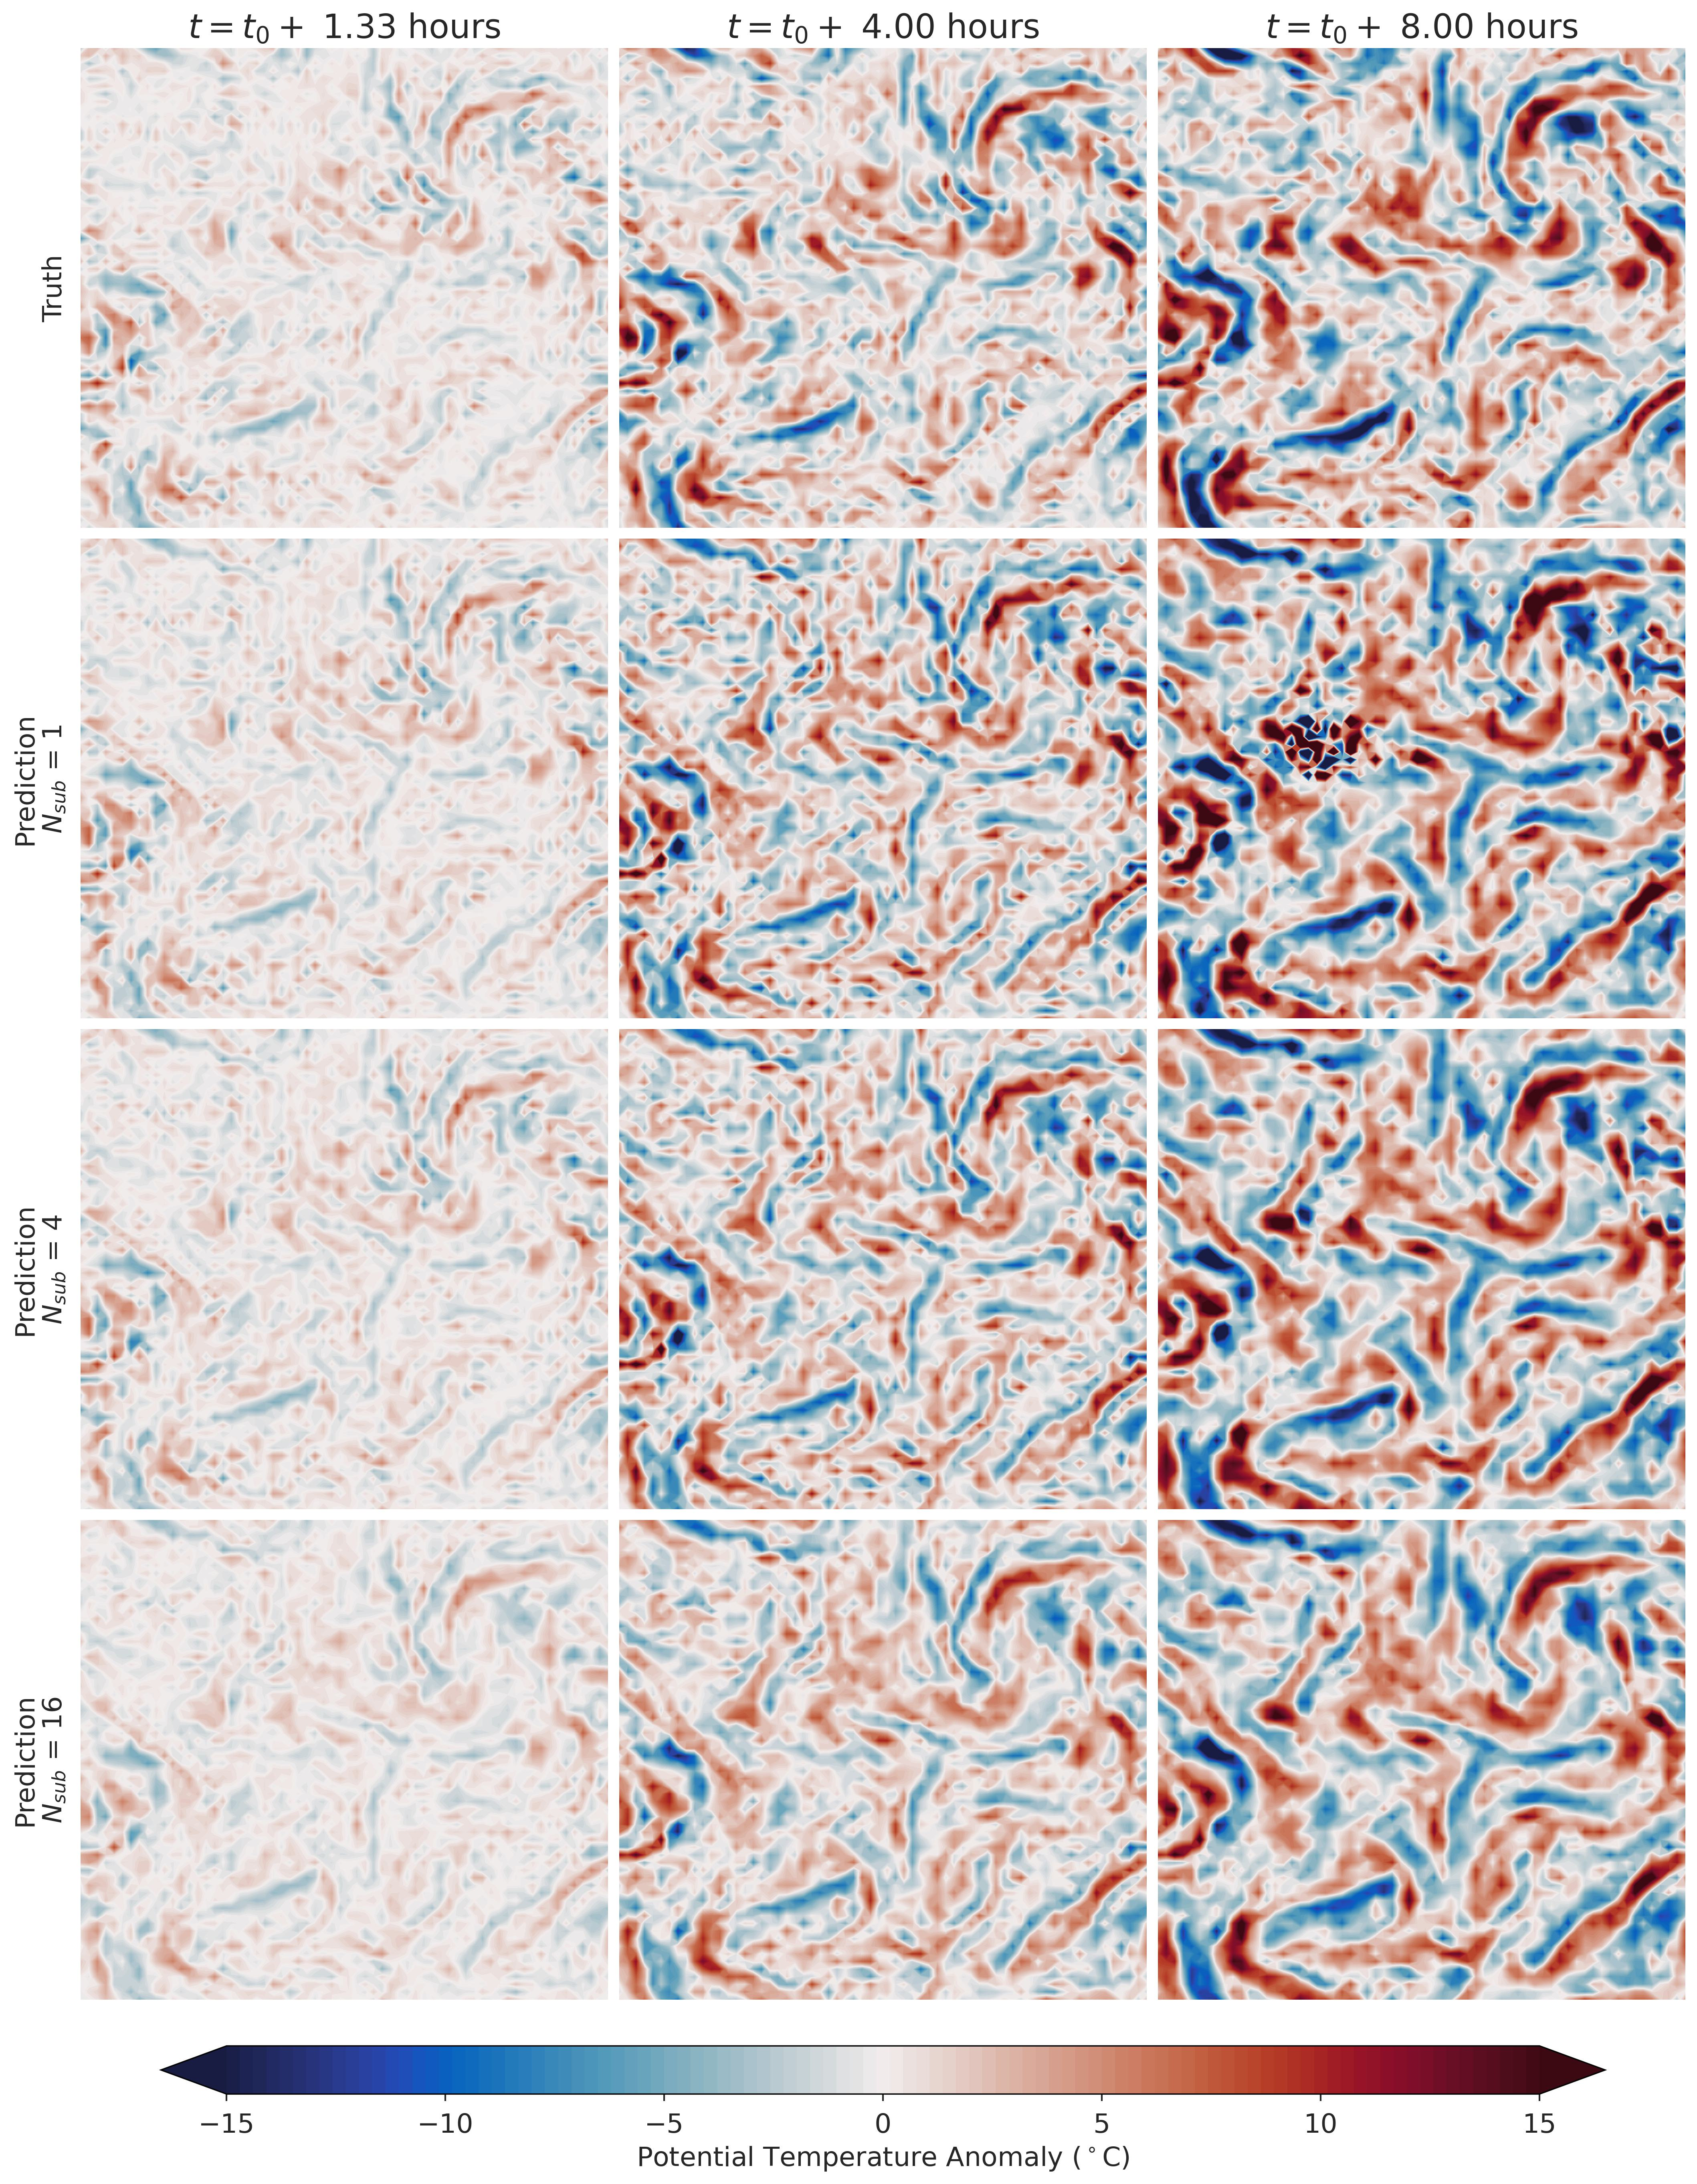
\includegraphics[width=\textwidth]{../figures/nvar_big_plot.jpg}
    \caption{One sample NVAR prediction from the test dataset for $\nsub =
        1,4,16$, shown in the second, third, and fourth rows.
        The corresponding truth is shown in the top row.
        In order to emphasize the changing features in the plot, each panel
        shows the difference between the state after 1.33, 4, and 8 hours with
        the initial conditions ($t_0$), corresponding to the left, middle, and
        right columns.
        Here $\maxlag=1$.
    }
    \label{fig:nvar_qualitative}
\end{figure}

\begin{figure}
    \centering
    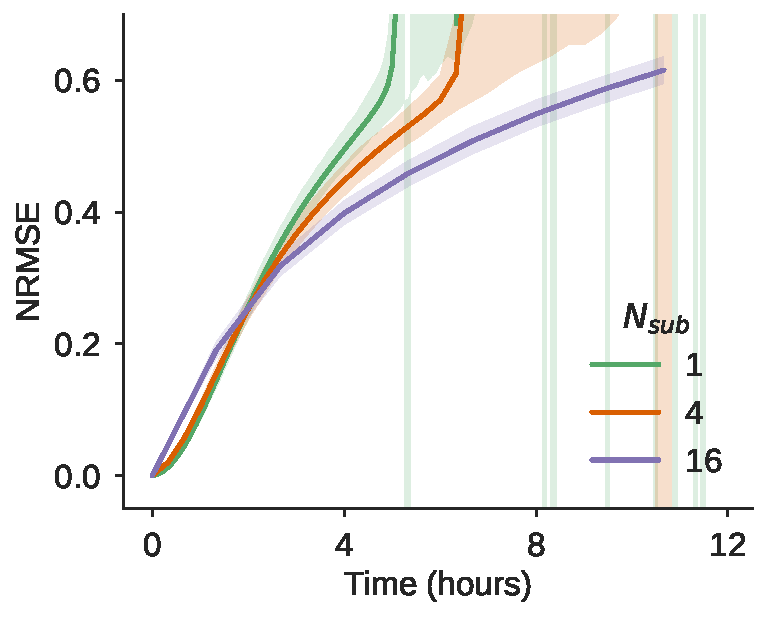
\includegraphics[width=.4\textwidth]{../figures/nvar_nrmse.pdf}
    \caption{Normalized Root-Mean-Square Error (NRMSE)
        indicating prediction skill of the NVAR
        architecture using 50~samples from the test dataset.
        Solid lines indicate averages and spread indicates 99\% confidence
        interval.
        Here $\nlag=1$.
    }
    \label{fig:nvar_nrmse}
\end{figure}

% Describe the big plot
% diff btwn t0, Nlag=1, one sample from test dataset
\cref{fig:nvar_qualitative} shows a qualitative comparison of NVAR predictions
as a function of $\nsub$, i.e., how frequently the training data are sampled and
the model makes predictions.
Each panel shows the difference between a given timestep and the initial
conditions in order to emphasize the features that change over an 8~hour window.
The top row shows the truth, while subsequent rows show the evolution of NVAR
predictions for $\nsub=1,4,16$.
For this figure, we set $\nlag=1$, and note that the normalized root-mean-square
error (NRMSE) corresponding to this configuration is shown in
\cref{fig:nvar_nrmse},
indicating prediction skill across 50~samples in the test dataset.
NRMSE at each timestep $n$ and for each sample is computed as follows
\begin{linenomath*}\begin{equation}
    \text{NRMSE}(n) = \sqrt{\dfrac{1}{\nstate}\sum_{i=1}^{\nstate}\left(
        \dfrac{\hat{v}_i(n) - v_i(n)}{SD}
        \right)^2 }
\end{equation}\end{linenomath*}
where for simplicity $i$ is an index for all spatial dimensions in 3D space,
and $SD$ is the standard deviation of the truth sample, computed over all
spatial dimensions and across time.

% Describe qualitatively what happens as we subsample the data further
% At Nsub=1, unstable, some smoothness especially at longer times but less so at
% short times
% As Nsub increases, stable, but "more smooth" at small scales even at shorter
% prediction windows
At the model timestep ($\Delta \tau = \Delta t = 5$~min; $\nsub=1$), the NVAR predictions are
qualitatively similar to the truth for relatively short forecast windows.
That is, the NRMSE is near 0, and
many of the fronts and dipoles that exist in the truth are also evident
in the predictions.
However, at longer forecast windows the predictions are unstable: NRMSE spikes
rapidly after about 4~hours and in \cref{fig:nvar_qualitative} instabilities are
present after 8~hours.

%Additionally, as the forecast develops, the prediction becomes somewhat smoother
%than the truth, which is evident as many small scale features are connected in
%the prediction.
As the temporal resolution of the data is reduced, i.e., as $\nsub$ increases,
the predictions are generally stable for a longer period of time.
\cref{fig:nvar_nrmse} shows that for $\nsub=4$, predictions are stable for roughly
6~hours, and for $\nsub=16$ no predictions generate numerical instabilities over the
12~hour window.
However, this stability comes with a cost: as the temporal resolution is
reduced, the model's representation of small scale features diminishes as these
features become more blurry or smooth.
This blurring effect is apparent in \cref{fig:nvar_qualitative}, where at each
timestep (column), the prediction is progressively more blurry at larger values
of $\nsub$.
At $\nsub=16$ ($\Delta \tau = $1.33~hrs), the smoothing effect is
evident even after a single timestep (i.e., the first column in
\cref{fig:nvar_qualitative}),
as many small scale features are broader than the truth and fronts generally
exhibit lower amplitudes.


% To show a quantitative discussion, consider the relative error in the KE density
% First column only: colors show error at different time stamps, spread
% indicates error over 50 samples in test dataset,
% In all plots, error is largest at the small spatial scales, corresponding to
% larger wavenumbers
% Note that not all of the Nsub=1,4 sims are stable, so the relative error is
% unacceptably large for t0+8 hrs, well beyond what is shown...
This smoothing behavior is captured quantitatively in \cref{fig:nvar_spectra},
which shows the relative error in terms of the kinetic energy density spectrum
and as a function of forecast time (panels) and $\nsub$ (colors).
The solid lines indicate average error and the shading indicates the 99\%
confidence interval, computed based on 50~samples predictions each initialized
from different initial conditions in the test dataset.
Generally speaking, error is largest in all cases at smaller spatial scales,
which corresponds to the higher wavenumbers.
%Note also that not all of the predictions produced with $\nsub=\{1,4\}$ are
%stable, so the relative error is \red{unacceptably large} after 8~hours, and
%therefore not shown.

% Nsub=1,4 produce nearly identical errors at small scales for short lead times,
% Nsub 1 generates instabilities in many simulations early on, and so error is
% large
% by subsampling the data more dramatically, Nsub=16, we see the error in the
% small scales grows considerably (by at least 40%).
At short lead times, the relative error is smallest and nearly
identical for $\nsub=\{1,4\}$.
However, as discussed above,
these predictions generate instabilities rapidly, and so the relative error is
greater than one by 8~hours.
By increasing the subsampling factor to $\nsub=16$, the simulations are stable
and relative error is less than or equal to one.
However, at all timesteps shown the relative error is 2-3 times larger for
$|\mathbf{K}| > 4\cdot10^{-3}$~rad~km$^{-1}$.
This error at higher wavenumbers corresponds to the qualitatively smooth
prediction shown in \cref{fig:nvar_qualitative}, as the small spatial scale
features are simply not resolved.

\begin{figure}
    \centering
    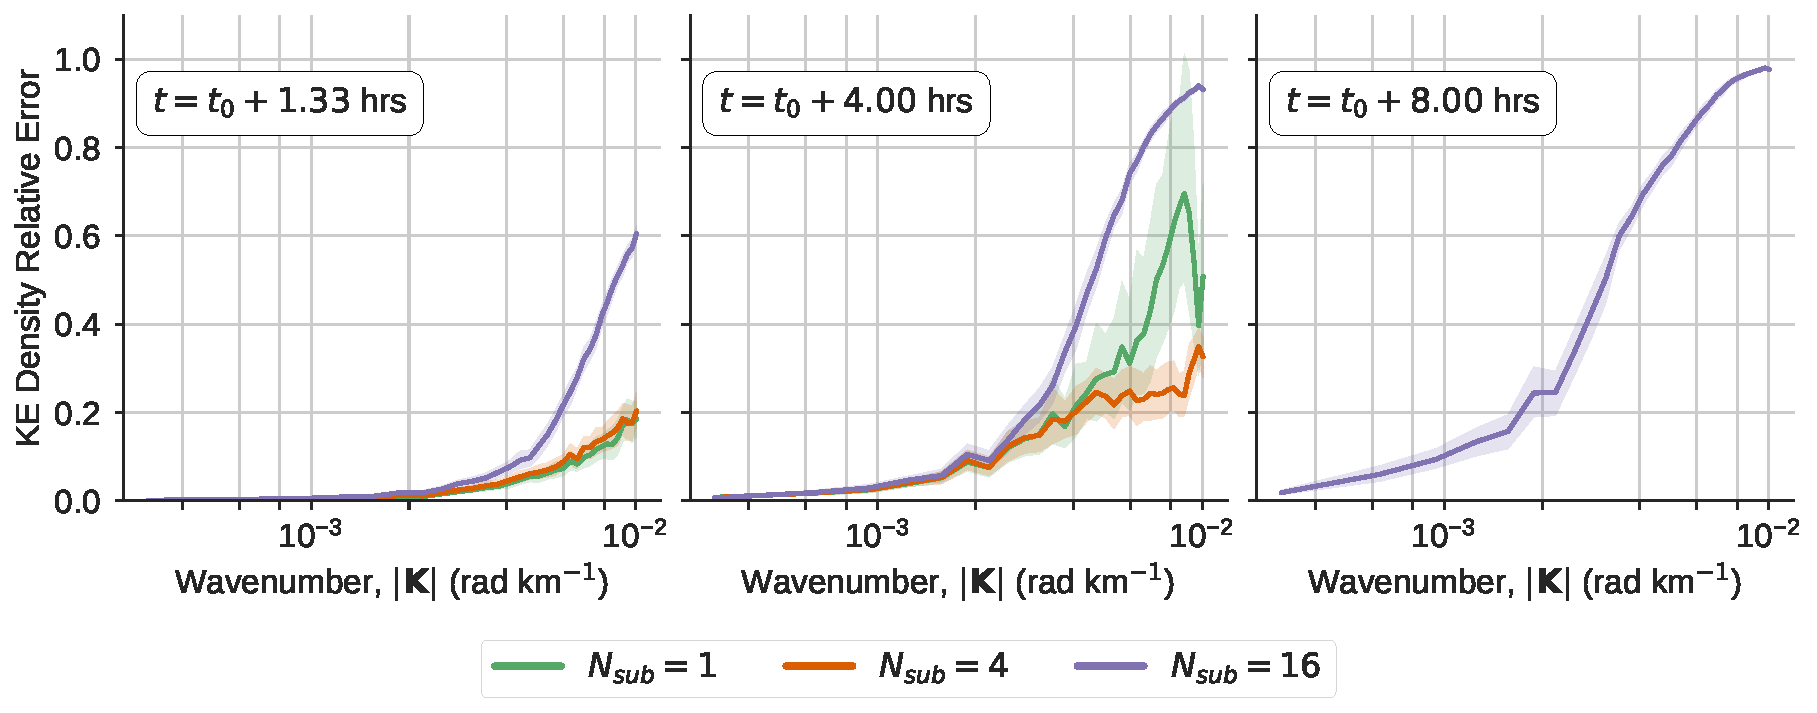
\includegraphics[width=\textwidth]{../figures/nvar_ke_relerr.pdf}
    \caption{Kinetic energy density relative error as a function of time
        (columns) and temporal resolution ($\nsub$; colors).
        Each line indicates error computed over 50~samples from the test
        dataset where solid lines indicate average error and shading indicates
        the 99\% confidence interval.
    }
    \label{fig:nvar_spectra}
\end{figure}


\subsubsection{Prediction Skill as a Function of Memory}

% A key feature of RNNs and autoregressive models is memory
% NVAR gives us the opportunity to explore this explicitly.
A key feature of RNNs and autoregressive models is that they retain memory of
previous system states.
Given the explicit nature of the NVAR architecture, we explore the effect of
adding memory by increasing $\nlag$, the number of lagged states used to create the
feature vector.
We first summarize how memory impacts prediction skill in
\cref{fig:nvar_nrmse_vs_lag}, which shows the NRMSE as a
function of $\nlag$ (colors) for each
subsampling factor $\nsub = \{1, 4, 16\}$ (panels).
For any value of $\nsub$, adding memory (increasing $\nlag$) reduces
the short term error.
However, adding memory also tends to increase error by the end of the forecast,
and often leads to the development of numerical instabilities and an
incoherent solution.
Similarly, for any fixed value of $\nlag$, increasing the temporal resolution
(decreasing $\nsub$) shows the same behavior.

\begin{figure}
    \centering
    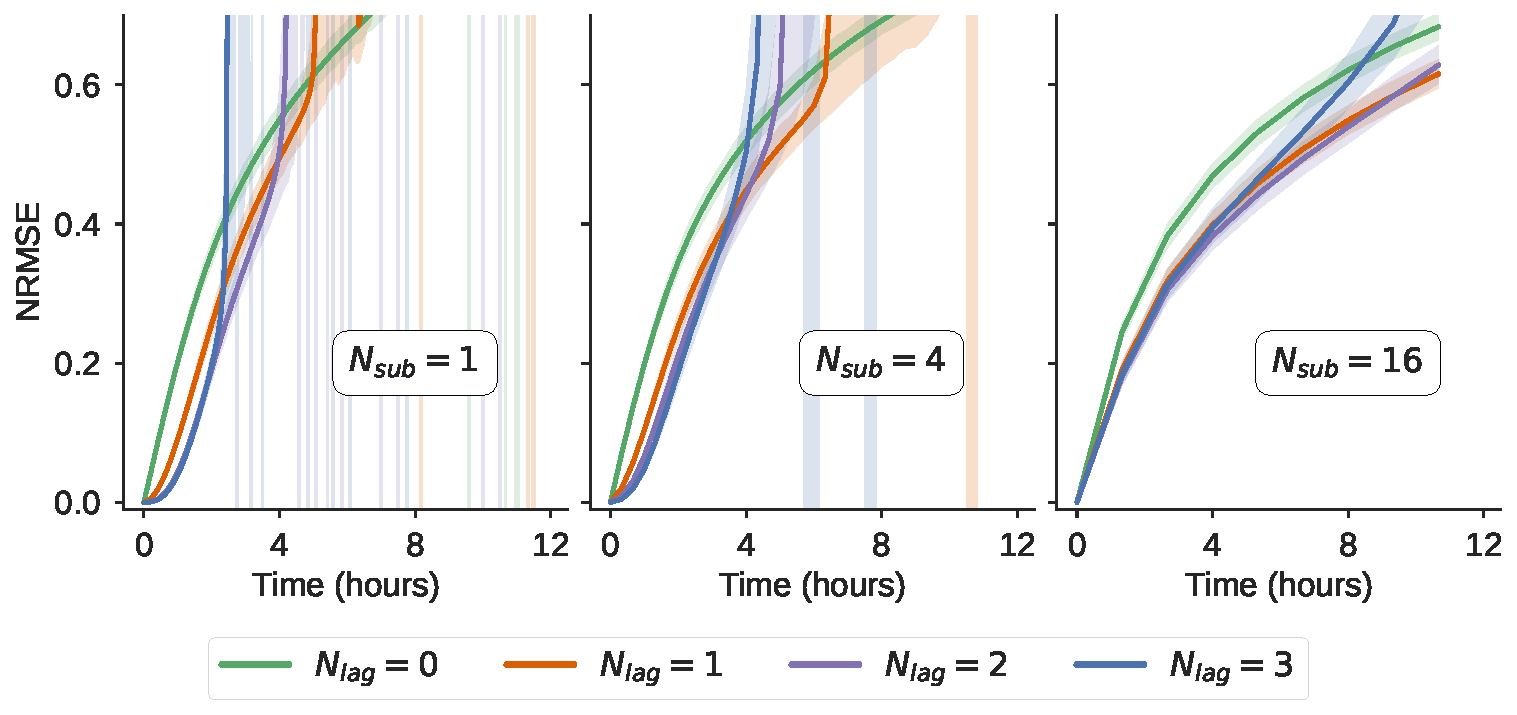
\includegraphics[width=\textwidth]{../figures/nvar_nrmse_vs_memory.pdf}
    \caption{NRMSE computed using NVAR at various temporal resolutions
        ($\nsub$; columns) and with variable memory capacities ($\nlag$;
        colors).
        Error is computed over 50~samples from the test dataset; solid lines
        indicate averages and shading indicates the 99\% confidence
        interval.
    }
    \label{fig:nvar_nrmse_vs_lag}
\end{figure}

To shed some light on how this additional memory impacts the solution,
we show the kinetic energy relative error
for the case of $\nsub=16$ as a function of time (panels) and $\nlag$ (colors)
in \cref{fig:nvar_ke_vs_lag}.
For about the first 4~hours, prediction skill is improved at all spatial scales.
However, beyond this point, the overall NRMSE grows rapidly, the improvement
at small scales ($|\mathbf{K}|>4\cdot10^{-3}$~rad~km$^{-1}$) is more muted,
and error is propagated rapidly into the larger spatial scales.

\red{given the performance of a purely linear NVAR model},
we surmise that adding memory degrades the long term prediction skill because
the relationship between points further back in history are governed by higher
order nonlinear interactions that are incorrectly represented by
the simple quadratic relation that is used here.
As more terms are added that are incorrectly represented, the model becomes
more and more unstable.
The question is therefore how to retain the short term benefit of added memory
capacity throughout the forecast horizon while maintaining a stable trajectory.
While it may seem natural to explore higher order polynomials to
properly represent this history, we do not explore this further because the size
of the feature vector grows dramatically with the polynomial order
\citep{chen_next_2022}.
Another option would be to explore entirely different basis functions.
While this could be a potential option for future work, we note the findings of
\citet{zhang_catch-22_2022}, who show the extreme sensitivity of NVAR to the
form of nonlinearity imposed.
Given that it is an entirely open question on how to represent the smallest
scales of geophysical turbulence, we do not explore other basis functions, and
instead turn to the more general RC architecture.
\todo{ask for TC's comments on this Paragraph}

\begin{figure}
    \centering
    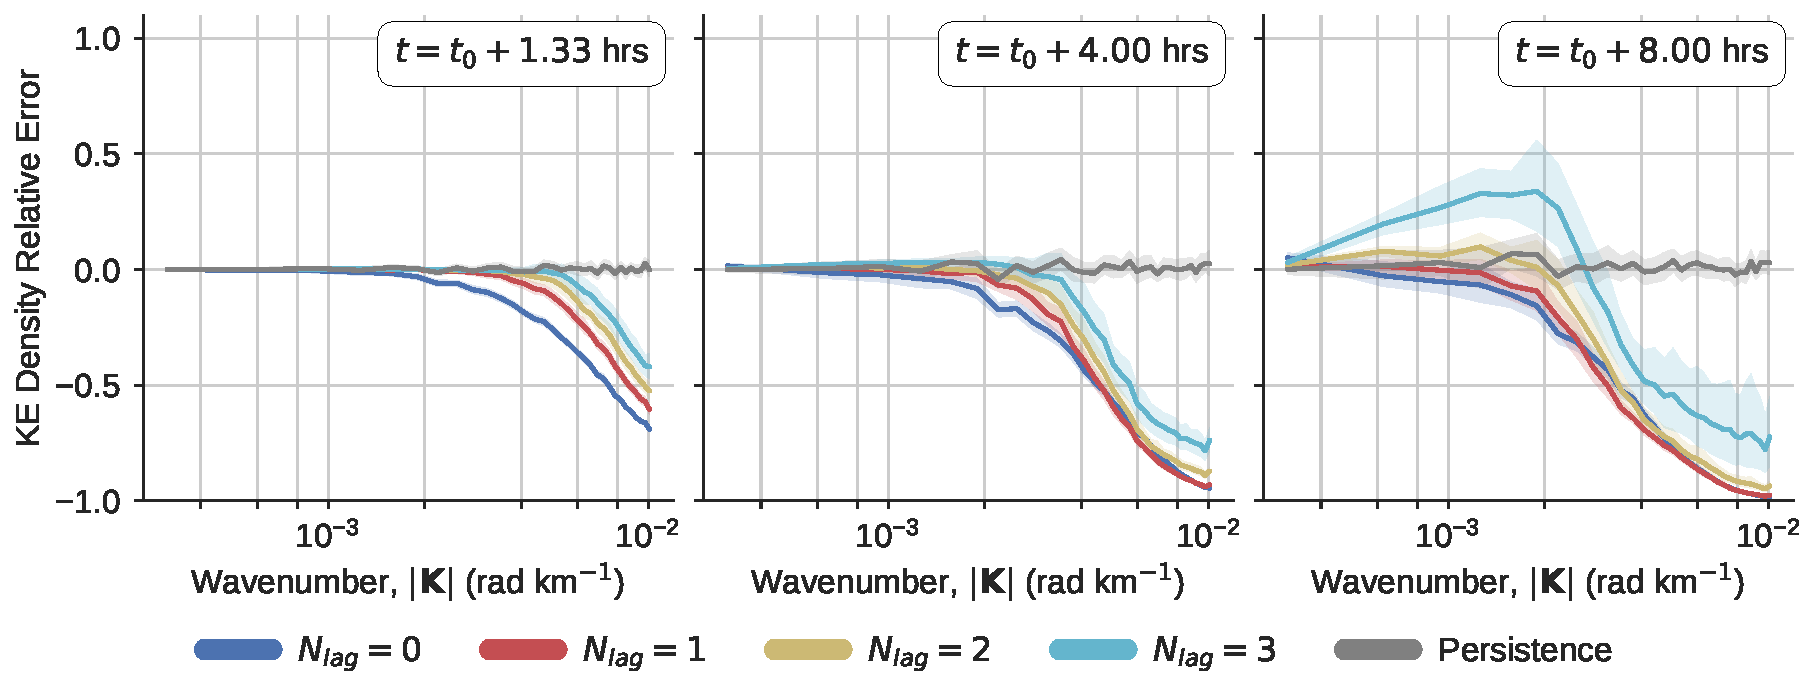
\includegraphics[width=\textwidth]{../figures/nvar_ke_relerr_vs_lag.pdf}
    \caption{Kinetic energy density relative error with $\nsub=16$ at various
        timesteps (columns) and memory capacity ($\nlag$; colors).
        Error is shown from 50~samples from the test dataset, indicating average
        and 99\% confidence interval.
    }
    \label{fig:nvar_ke_vs_lag}
\end{figure}
